\chapter{ВЕРИФИКАЦИЯ И РЕАЛИЗАЦИЯ УСТРОЙСТВА}
\label{cha:impl}

В данном разделе будет представлена практическая часть НИР, а именно верификация работы и реализация цифровой схемы устройства на ПЛИС.

\section{Верификация}

Для моделирования работы системы было реализовано тестовое окружение для формирования тестовых воздействий на модули управления устройства. При помощи системы моделирования Questa Sim были построены временные диаграммы работы устройства. На рисунке \ref{fig:verification_all} показан общий вид временной диаграммы.


\begin{figure}[ht]
    \centering
    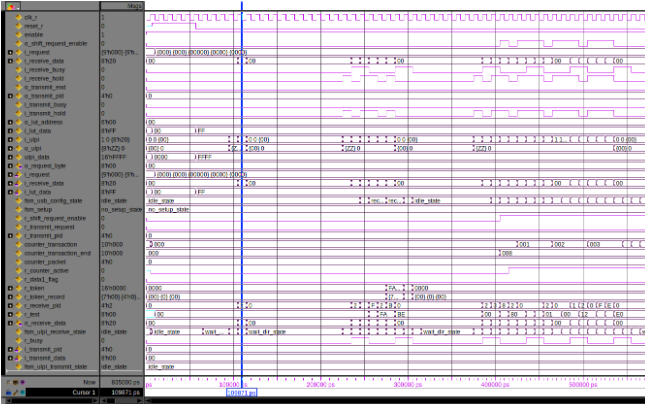
\includegraphics[scale=0.7]{res/img/verification_all.png}
    \caption{Общий вид временной диаграммы}
    \label{fig:verification_all}
\end{figure}

\pagebreak
На рисунке \ref{fig:verification_setup} представлена диаграмма отправки токена SETUP на модуль блока конфигурации. Данные помещаются в регистры, соответствующие их назначению в протоколе: сравниваются адрес, конечная точка и контрольная сумма CRC5. Модуль корректно обрабатывает задержки со стороны устройства при установке \detokenize{i_ulpi.nxt} в логический 0. При этом вход двунаправленной шины данных помещается в высокоимпедансное состояние Z для избежания конфликтов на шине.

\begin{figure}[ht]
    \centering
    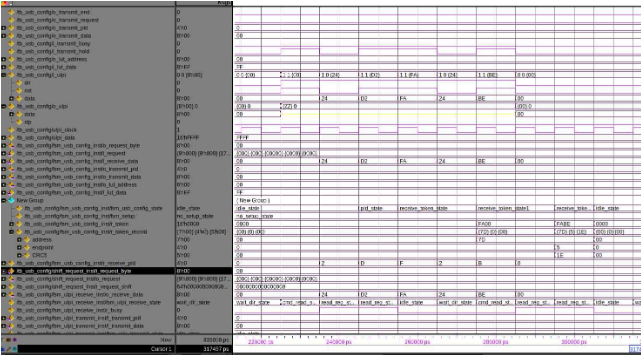
\includegraphics[scale=0.7]{res/img/verification_setup.png}
    \caption{Диаграмма отправки токена SETUP}
    \label{fig:verification_setup}
\end{figure}

\pagebreak
На рисунке \ref{fig:verification_data0} изображена диаграмма передачи длинного сообщения DATA0.

\begin{figure}[ht]
    \centering
    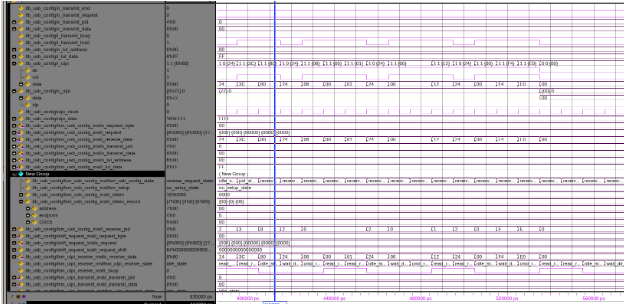
\includegraphics[scale=0.7]{res/img/verification_data0.png}
    \caption{Диаграмма отправки токена DATA0}
    \label{fig:verification_data0}
\end{figure}

На рисунке \ref{fig:verification_ack} изображена диаграмма передачи короткой квитанции ACK подтверждения сообщения.


\begin{figure}[ht]
    \centering
    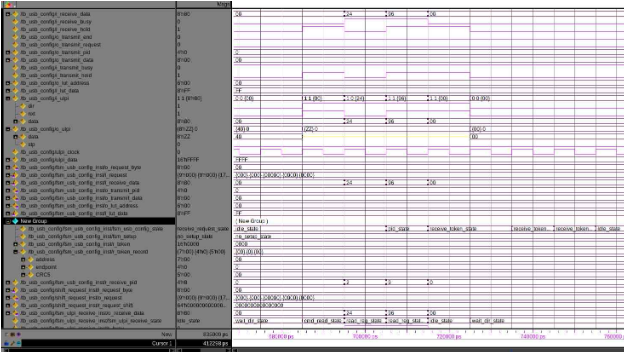
\includegraphics[scale=0.7]{res/img/verification_ack.png}
    \caption{Диаграмма отправки токена ACK}
    \label{fig:verification_ack}
\end{figure}


\section{Практическая реализация}

Был выполнен синтез проекта на ПЛИС GoWin GW1NR-9 в среде GoWin EDA. На рисунке \ref{fig:synth_report} представлены результаты проведённого синтеза и отчёт о занимаемых ресурсах. Все этапы синтеза пройдены успешно. На рисунке \ref{fig:synth_rtl} показана синтезированная схема модуля.

\begin{figure}[ht!]
    \centering
    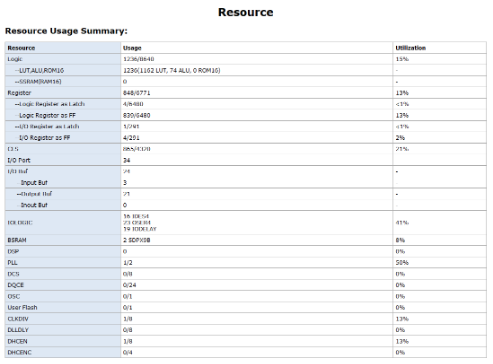
\includegraphics[scale=0.7]{res/img/synth_report.png}
    \caption{Отчёт о занимаемых ресурсах}
    \label{fig:synth_report}
\end{figure}


\begin{figure}[ht!]
    \centering
    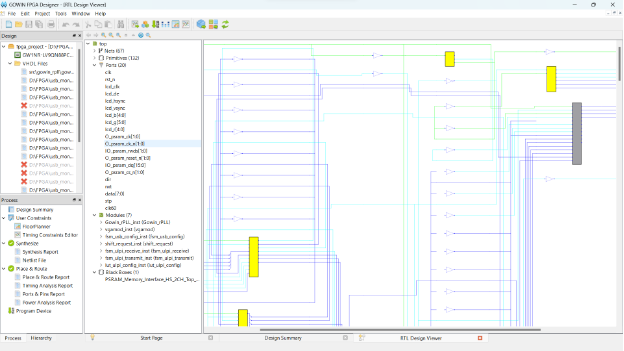
\includegraphics[scale=0.7]{res/img/synth_rtl.png}
    \caption{Синтезируемая схема модуля}
    \label{fig:synth_rtl}
\end{figure}

\begin{figure}[ht!]
    \centering
    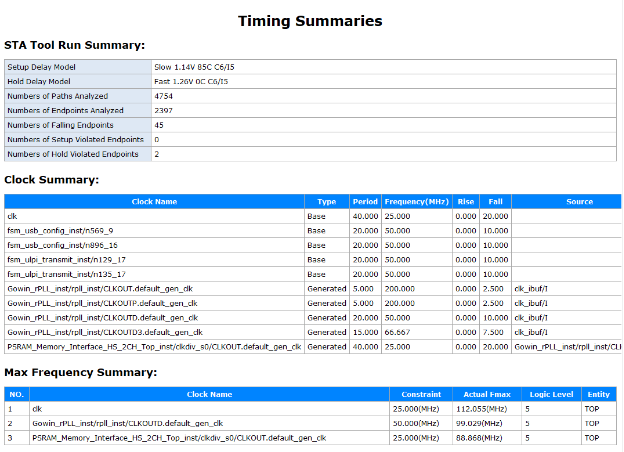
\includegraphics[scale=0.7]{res/img/synth_timing.png}
    \caption{Отчёт о временных характеристиках модуля}
    \label{fig:synth_timing}
\end{figure}



Временных характеристик искомой ПЛИС оказалось достаточно для реализации данного проекта, все временные требования к тактовым сигналам и делителям частоты были соблюдены, что отражено в отчёте, отображённом на рисунке \ref{fig:synth_timing}.
